% Промежуточный доклад (M-talk). Компиляция: cd slides && xelatex midterm.tex
% Рисунки берутся из ../figures (их строит code/plots.py), слайды извлечены из статьи paper/main.tex
\documentclass[aspectratio=169,10pt]{beamer}
\usepackage{fontspec}
\usepackage{polyglossia}
\setdefaultlanguage{russian}
\setotherlanguage{english}
\setmainfont{DejaVu Sans}
\setsansfont{DejaVu Sans}
\setmonofont{DejaVu Sans Mono}
\newfontfamily\condensed{DejaVu Sans Condensed}
\usepackage{unicode-math}
\setmathfont{Latin Modern Math}
\usepackage{graphicx}
\usepackage{booktabs}
\usepackage{array}

\definecolor{ink}{HTML}{0B0B0B}
\definecolor{ink2}{HTML}{52514E}
\definecolor{accent}{HTML}{1C5CAB}
\definecolor{soft}{HTML}{EEF4FC}
\setbeamertemplate{navigation symbols}{}
\setbeamercolor{normal text}{fg=ink}
\setbeamercolor{frametitle}{fg=accent}
\setbeamercolor{structure}{fg=accent}
\setbeamerfont{frametitle}{size=\large,series=\bfseries}
\setbeamertemplate{itemize items}{\color{accent}\textbullet}
\setbeamersize{text margin left=7mm,text margin right=7mm}
\setbeamertemplate{frametitle}{\vspace*{2mm}\insertframetitle\par
  \ifx\insertframesubtitle\empty\else{\normalfont\fontsize{8.5}{10}\selectfont\color{ink2}\insertframesubtitle\par}\fi}
\setbeamertemplate{footline}{\hbox to \paperwidth{\hspace*{7mm}\fontsize{6}{7}\selectfont\color{ink2}%
  ВМК МГУ\enspace·\enspace «Моя первая научная статья», 2026\enspace·\enspace промежуточный доклад%
  \hfill\insertframenumber/\inserttotalframenumber\hspace*{7mm}}\vspace*{2mm}}

\newcommand{\head}[1]{{\fontsize{9}{10.5}\selectfont\color{accent}\bfseries #1}\par\vspace{0.6mm}}
\newcommand{\txt}{\fontsize{8.5}{10.2}\selectfont}
\DeclareMathOperator{\Var}{Var}
\newcommand{\colfont}{\condensed\fontsize{7.4}{8.8}\selectfont}
\newcommand{\thesis}[1]{\par\vspace{1mm}{\bfseries\color{accent}#1}\ }
\newcommand{\key}[1]{{\color{accent}\bfseries #1}}

\begin{document}

%————————————————————-- 1
\begin{frame}[plain]
\vspace{14mm}
{\fontsize{17}{21}\selectfont\bfseries\color{accent}
Сколько попарных сравнений\\ заменяют признаки объектов\par}
\vspace{2mm}
{\fontsize{11}{14}\selectfont\color{ink2}Априорный прогноз для иерархической модели Брэдли--Терри\par}
\vspace{9mm}
{\txt
Минабутдинов Камиль\\[1mm]
ВМК МГУ, кафедра ММП\par}
\vspace{9mm}
\begin{beamercolorbox}[wd=\linewidth,sep=2.5mm]{}
\colorbox{soft}{\parbox{0.96\linewidth}{\vspace{1.5mm}\txt
\key{Цель:} до проведения опроса предсказать, во сколько раз признаки объектов сокращают число попарных сравнений, нужных людям для ранжирования. Пример применения — выбор татарской замены русского заимствования по мнению носителей.\vspace{1.5mm}}}
\end{beamercolorbox}
\end{frame}

%————————————————————-- 2  (обновлённый O-слайд)
\begin{frame}[t]
\frametitle{Признаки заменяют часть опроса носителей}
\vspace{-1mm}
\begin{columns}[T,onlytextwidth]
\begin{column}{0.30\textwidth}\colfont\raggedright
\head{Что и зачем}
\thesis{Задача.} Упорядочить замены слова по сравнениям «какая лучше».
\thesis{Проблема.} Носителей мало, опрос дорог.
\thesis{Идея.} Признаки слова дают априорную оценку, сравнения её уточняют.
\thesis{Результат.} Формула пересчитывает признаки в число сравнений до опроса.
\end{column}
\begin{column}{0.68\textwidth}\centering
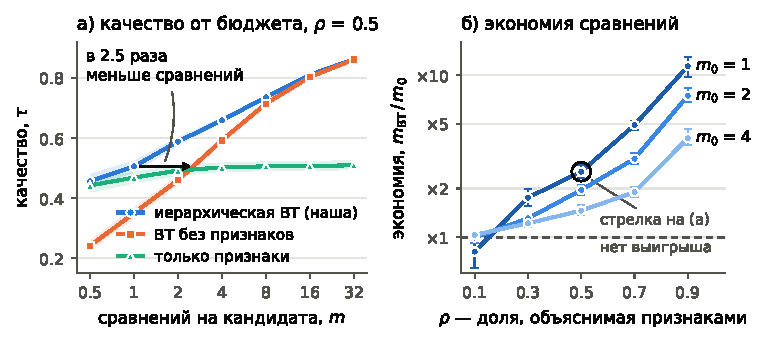
\includegraphics[width=0.97\linewidth]{../figures/main_figure_slide.pdf}
\end{column}
\end{columns}
\vspace{3mm}
\begin{columns}[T,onlytextwidth]
\begin{column}{0.34\textwidth}\colfont\raggedright
\head{Модель}
$P(i\succ j)=\sigma(u_i-u_j)$,\ \ $u_i=\theta^{\top}\mathbf x_i+\eta_i$;\\
$\rho$ — доля разброса предпочтений, объяснимая признаками.
\end{column}
\begin{column}{0.33\textwidth}\colfont\raggedright
\head{Формула экономии}
$\displaystyle \frac{m_{\mathrm{BT}}}{m_0}=1+\frac{K-1}{K\bar I V}\cdot\frac{\rho}{(1-\rho)\,m_0}$\\[0.5mm]
уточнённый прогноз Монте-Карло точен до 5\,\%.
\end{column}
\begin{column}{0.30\textwidth}\colfont\raggedright
\head{Проверка на людях}
Оценки сложности слов от 11 человек: прогноз верно упорядочивает признаки по силе ($r_s=0{,}96$), но завышает экономию.
\end{column}
\end{columns}
\end{frame}

%————————————————————-- 3
\begin{frame}[t]
\frametitle{Литература: что известно и чего не хватает}
\vspace{1mm}
{\txt
\begin{tabular}{@{}>{\raggedright\arraybackslash}p{0.33\textwidth}>{\raggedright\arraybackslash}p{0.62\textwidth}@{}}
\toprule
\textbf{Работа} & \textbf{Что даёт нам} \\
\midrule
Bradley, Terry, 1952 & модель выбора в паре — базовый метод \\
Springall, 1973; Turner, Firth, 2012 & модель с признаками и случайным эффектом объекта — наша модель \\
Chu, Ghahramani, 2005 & байесовская модель предпочтений с лапласовым приближением \\
Shah и др., 2016 & ошибка без признаков определяется спектром графа сравнений \\
Morita и др., 2008 & эффективный размер выборки априорного распределения — ближайшая идея \\
Angelopoulos и др., 2023; Chatzi и др., 2024 & как объединять ответы людей с предсказаниями моделей \\
\bottomrule
\end{tabular}}
\vspace{4mm}

\colorbox{soft}{\parbox{0.97\linewidth}{\vspace{1.2mm}\txt
\key{Пробел:} нет правила, переводящего информацию признаков в \emph{число сравнений} при заданном плане опроса и вычислимого \emph{до} сбора данных.\vspace{1.2mm}}}
\end{frame}

%————————————————————-- 4
\begin{frame}[t]
\frametitle{Постановка задачи}
\vspace{1mm}
\begin{columns}[T,onlytextwidth]
\begin{column}{0.49\textwidth}\txt\raggedright
\head{Данные}
$G$ групп по $K$ объектов (заимствование и его замены), признаки $\mathbf x_i\in\mathbb R^d$. План опроса $q$ — распределение на парах внутри групп; бюджет $m$ — сравнений на объект.

\vspace{2mm}\head{Гипотезы}
$P(i\succ j)=\sigma(u_i-u_j)$;\quad $u_i=\theta^{\top}\mathbf x_i+\eta_i$,\ \ $\eta_i\sim\mathcal N(0,(1-\rho)V)$,\\[0.5mm]
$\rho=\Var(\theta^{\top}\mathbf x)/\Var(u)$.

\vspace{2mm}\head{Модель и внутренний критерий}
$\displaystyle\min_{\theta,\eta}\ -\sum_t\log\sigma(s_{w_t}-s_{l_t})+\tfrac{\lambda}{2}\|\eta\|^2+\tfrac{\lambda_\theta}{2}\|\theta\|^2$,\\[0.5mm]
$s=X\theta+\eta$. Базовые: BT ($\theta=0$), «только признаки» ($\eta=0$).
\end{column}
\begin{column}{0.47\textwidth}\txt\raggedright
\head{Внешние критерии}
$\tau$ Кендалла внутри групп; доля верно найденных лучших (top-1); правдоподобие контрольных сравнений; MSE внутригрупповых контрастов.

\vspace{2mm}\head{Исследуемая величина}
Эквивалентный бюджет и экономия:
\[
m_{\mathrm{BT}}(m_0)=\min\{m:\ \mathcal Q_{\mathrm{BT}}(m)\ge\mathcal Q_{\mathrm H}(m_0)\},
\]
\[
\kappa=m_{\mathrm{BT}}/m_0.
\]
\colorbox{soft}{\parbox{0.95\linewidth}{\vspace{1mm}
\key{Задача:} прогноз $\hat\kappa(m_0;\rho,V,K,q)$ до сбора данных и оценка его точности.\vspace{1mm}}}
\end{column}
\end{columns}
\end{frame}

%————————————————————-- 5
\begin{frame}[t]
\frametitle{Решение: три утверждения и алгоритм прогноза}
\framesubtitle{Лапласово приближение: риск $R(L,a)=\frac1N\operatorname{tr}\bigl(C(L+aI)^{-1}\bigr)$, $L$ — лапласиан графа сравнений, $a$ — априорная точность}
\vspace{0.5mm}
\begin{columns}[T,onlytextwidth]
\begin{column}{0.50\textwidth}\txt\raggedright
\head{Теорема 1 (случайные пары)}
\[
m_{\mathrm{BT}}=m_0+\frac{K-1}{K\,\bar I\,V}\cdot\frac{\rho}{1-\rho},\qquad \bar I=\mathbb E\,\sigma'(D).
\]
Признаки равносильны лишним сравнениям каждому объекту.

\vspace{1.5mm}\head{Теорема 2 (любой план)}
$\Delta_k=\dfrac{\rho}{(1-\rho)V\mu_k}$ по собственным числам $\mu_k$:\\[0.5mm]
$m_0+\min\Delta_k\le m_{\mathrm{BT}}\le m_0+\max\Delta_k$.\\
\key{Признаки ценнее при разреженном опросе.}
\end{column}
\begin{column}{0.46\textwidth}\txt\raggedright
\head{Теорема 3 (нижняя оценка)}
$\mathbb E\,R(L,a)\ge R(\mathbb E L,a)$: формула со средней информацией занижает риск (выпуклость $\operatorname{tr}X^{-1}$, неравенство Йенсена).

\vspace{1.5mm}\head{Алгоритм: прогноз Монте-Карло}
\begin{enumerate}\setlength{\itemsep}{0.3mm}
\item сгенерировать $u\sim\mathcal N(0,VI)$ и план опроса;
\item посчитать риск $R$ для BT и для модели с признаками на сетке $m$;
\item усреднить и решить $\bar R_{\mathrm{BT}}(m_{\mathrm{BT}})=\bar R_{\mathrm H}(m_0)$.
\end{enumerate}
Учитывает случайность плана и неравную информацию пар; 15~с на прогноз.
\end{column}
\end{columns}
\end{frame}

%————————————————————-- 6
\begin{frame}[t]
\frametitle{Эксперимент 1: прогноз против измерения (синтетика)}
\framesubtitle{40 групп по 8 объектов, $\rho\in\{0{,}1;\dots;0{,}9\}$, бюджеты до 128, 30 повторов, 95\,\%-е интервалы}
\vspace{-1mm}
\begin{columns}[T,onlytextwidth]
\begin{column}{0.64\textwidth}\centering
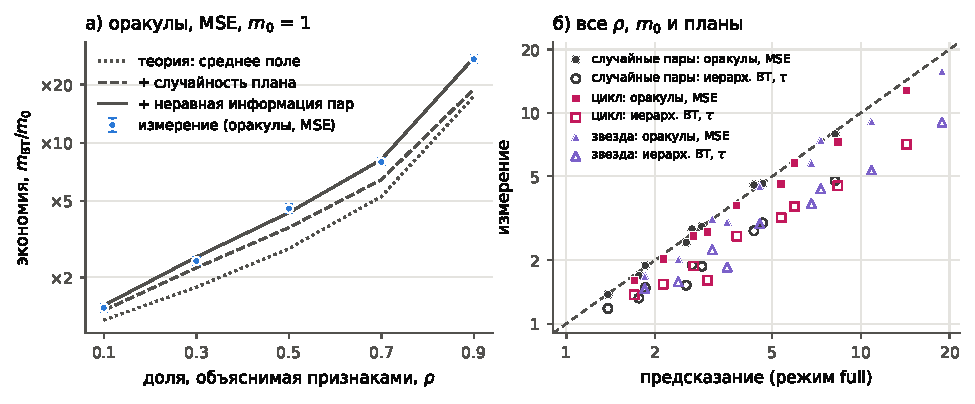
\includegraphics[width=\linewidth]{../figures/fig_theory_check.pdf}
\end{column}
\begin{column}{0.34\textwidth}\txt\raggedright
\vspace{2mm}
\head{Цель}
Проверить, что прогноз до эксперимента совпадает с измеренной экономией.

\vspace{1.5mm}\head{Результат}
\begin{itemize}\setlength{\itemsep}{0.6mm}
\item формула занижает экономию до 1,6 раза — как и следует из теоремы 3;
\item поправки на план ($\times$1,02–1,29) и информацию пар ($\times$1,03–1,46) дают прогноз, точный \key{до 5\,\%} во всех 15 ячейках;
\item цикл и звезда дают экономию в 1,6–2 раза больше случайных пар.
\end{itemize}
\end{column}
\end{columns}
\end{frame}

%————————————————————-- 7
\begin{frame}[t]
\frametitle{Эксперимент 2: реальные человеческие сравнения}
\framesubtitle{Замены слов BenchLS $\times$ оценки сложности 11 человек (WCL): 721 группа, 2641 слово, 74\,477 сравнений}
\vspace{-1mm}
\begin{columns}[T,onlytextwidth]
\begin{column}{0.55\textwidth}\centering
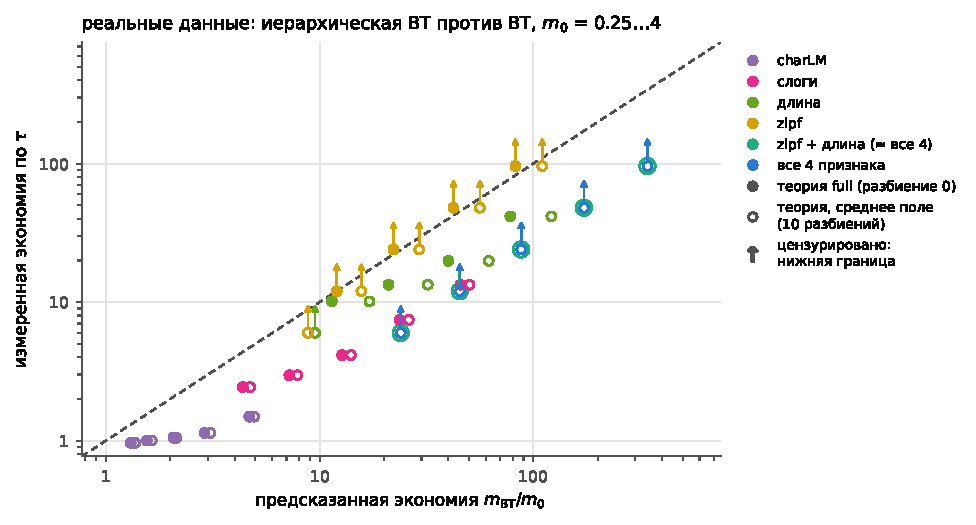
\includegraphics[width=\linewidth]{../figures/fig_real_theory.pdf}
\end{column}
\begin{column}{0.43\textwidth}\txt\raggedright
\vspace{1mm}
\head{Цель}
Проверить вывод на людях: структура как у татарских замен, а опрос носителей пока невозможен.

\vspace{1.5mm}\head{Результат}
\begin{itemize}\setlength{\itemsep}{0.6mm}
\item подсказки разной силы: символьная LM $\hat\rho=0{,}18$ $\to$ экономия ${\approx}1$; слоги $0{,}70\to\times4$; длина $0{,}84\to\times13$; частота $\to{>}\times24$;
\item прогноз верно упорядочивает подсказки: $r_s=0{,}96$;
\item но завышает экономию по $\tau$ в 1,1–3,4 раза (разные шкалы людей, ничьи).
\end{itemize}
\end{column}
\end{columns}
\end{frame}

%————————————————————-- 8
\begin{frame}[t]
\frametitle{Анализ ошибки}
\framesubtitle{Реальные данные: сложность модели и регуляризация}
\vspace{-1mm}
\begin{columns}[T,onlytextwidth]
\begin{column}{0.62\textwidth}\centering
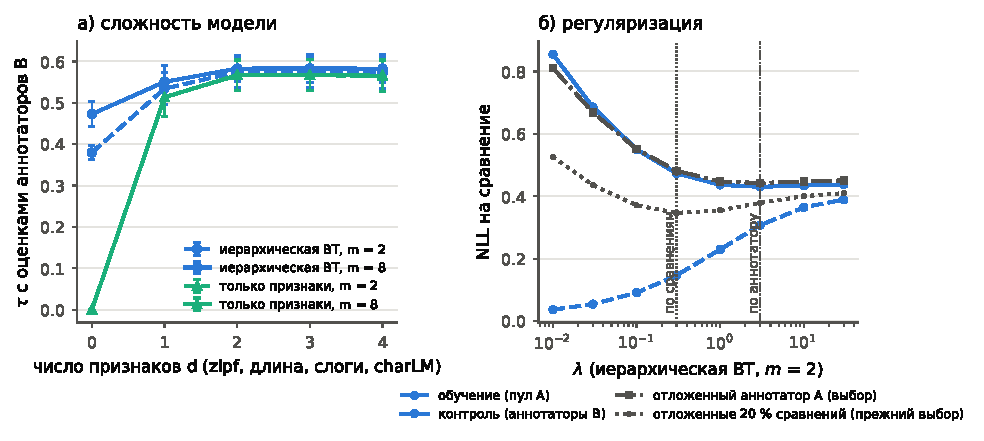
\includegraphics[width=\linewidth]{../figures/fig_complexity.pdf}
\end{column}
\begin{column}{0.36\textwidth}\txt\raggedright
\vspace{1mm}
\head{Сложность}
Почти весь эффект дают частота и длина; слоги и символьная LM ничего не добавляют.

\vspace{1.5mm}\head{Регуляризация — главный источник ошибки}
Если подбирать $\lambda$ по 20\,\% отложенных \emph{ответов}, модель подстраивается под шкалы тех же людей и ухудшается с ростом опроса.
Отложенный \emph{аннотатор} воспроизводит кривую контроля.\\[1mm]
\key{Вывод: параметры выбирать по отложенным людям.}
\end{column}
\end{columns}
\end{frame}

%————————————————————-- 9
\begin{frame}[t]
\frametitle{Итог: модели, данные, критерии}
\vspace{1mm}
{\txt\centering
\begin{tabular}{l cc ccc c}
\toprule
& \multicolumn{2}{c}{синтетика, $\rho=0{,}5$, $m=2$} & \multicolumn{3}{c}{реальные данные, $m=2$} & реальные, $m=8$ \\
\cmidrule(lr){2-3}\cmidrule(lr){4-6}\cmidrule(lr){7-7}
Модель & $\tau\uparrow$ & top-1\,$\uparrow$ & $\tau\uparrow$ & top-1\,$\uparrow$ & NLL\,$\downarrow$ & $\tau\uparrow$ \\
\midrule
BT без признаков & 0,460 & 0,349 & 0,380 & 0,522 & 0,564 & 0,473 \\
только признаки & 0,492 & 0,446 & 0,565 & 0,669 & 0,440 & 0,566 \\
иерархическая BT & \key{0,589} & \key{0,523} & \key{0,573} & \key{0,685} & \key{0,433} & \key{0,583} \\
\bottomrule
\end{tabular}\par}
\vspace{4mm}
\begin{columns}[T,onlytextwidth]
\begin{column}{0.50\textwidth}\txt\raggedright
\head{Выводы}
\begin{itemize}\setlength{\itemsep}{0.6mm}
\item формула пересчитывает признаки в число сравнений; уточнённый прогноз точен до 5\,\% в синтетике;
\item признаки ценнее всего при разреженном опросе;
\item на людях прогноз упорядочивает подсказки, но завышает выигрыш.
\end{itemize}
\end{column}
\begin{column}{0.46\textwidth}\txt\raggedright
\head{Дальше}
\begin{itemize}\setlength{\itemsep}{0.6mm}
\item татарские замены: признаки по корпусу, оценки LLM как подсказка;
\item поправка прогноза на ранговый критерий и разные шкалы людей;
\item прогноз для поиска лучшей замены, а не полного порядка.
\end{itemize}
\end{column}
\end{columns}
\end{frame}

\end{document}
